\documentclass[10pt,tikz,border=2mm]{standalone} 
\usepackage{mathpazo}
\usepackage[T1]{fontenc}
\usetikzlibrary{calc,positioning,arrows.meta}
\tikzstyle{arrow}=[-{Stealth[scale=2]},thin,text=black]
\begin{document}
	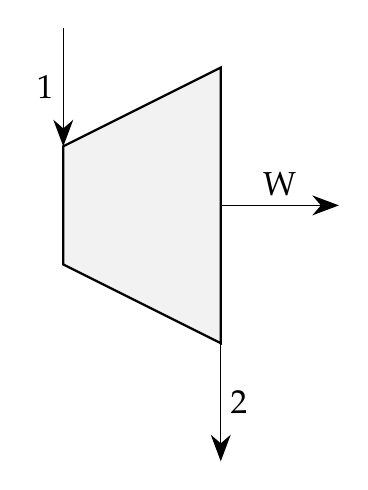
\begin{tikzpicture}[font=\large]
	%\draw[step=1cm,black!20,very thin] (0,0) grid (6,6);
	\coordinate (A) at (1,3.25);
	\coordinate (B) at (1,4.75);
	\coordinate (C) at (3,5.75);
	\coordinate (D) at (3,2.25);
	\coordinate (E) at ($(C)!0.5!(D)$);
	\coordinate (X) at (1.5,0);
	\coordinate (Y) at (0,1.5);
	\draw[thick,fill=black!5] (A)--(B)--(C)--(D)--cycle;
	\draw[arrow] ($(B)+(Y)$) -- node[left]{1} (B);
	\draw[arrow] (D) -- node[right]{2} ($(D)-(Y)$);
	\draw[arrow] (E) -- node[above]{W} ($(E)+(X)$);
	\end{tikzpicture}
\end{document}